\let\negmedspace\undefined
\let\negthickspace\undefined
\documentclass[a5paper,10pt]{article}
\usepackage[margin=10mm]{geometry}
%\usepackage{lmodern} % Ensure lmodern is loaded for pdflatex
\usepackage{tfrupee} % Include tfrupee package

\setlength{\headheight}{1cm} % Set the height of the header box
\setlength{\headsep}{0mm}     % Set the distance between the header box and the top of the text

\usepackage{gvv-book}
\usepackage{gvv}
\usepackage{cite}
\usepackage{amsmath,amssymb,amsfonts,amsthm}
\usepackage{algorithmic}
\usepackage{graphicx}
\usepackage{textcomp}
\usepackage{xcolor}
\usepackage{txfonts}
\usepackage{listings}
\usepackage{enumitem}
\usepackage{mathtools}
\usepackage{gensymb}
\usepackage{comment}
\usepackage[breaklinks=true]{hyperref}
\usepackage{tkz-euclide} 
\usepackage{listings}
% \usepackage{gvv}                                        
\def\inputGnumericTable{}                                 
\usepackage[latin1]{inputenc}                                
\usepackage{color}                                            
\usepackage{array}                                            
\usepackage{longtable}                                       
\usepackage{calc}                                             
\usepackage{multirow}                                         
\usepackage{hhline}                                           
\usepackage{ifthen}                                           
\usepackage{lscape}
\usepackage{circuitikz}



\author{EE25BTECH11041-Naman Kumar }
\graphicspath{./figs/}

\begin{document}
\begin{center}
    \huge{10.7.89}\\
    \large{EE25BTECH11041 - Naman Kumar}
\end{center}
Question:\\
Lines $5x + 12y - 10 = 0$ and $5x -12y - 40 = 0$ touch a Circle $C_1$ of diameter 6. If the centre of $C_1$ lies in the first quadrant, find the equation of circle $C_2$ which is concentric with $C_1$ and cuts intercepts of length 8 on these lines.\\
\solution \\
Given lines are tangents, their equations
\begin{align}
    \vec{n_1}\vec{x}=c_1,\vec{n_2}\vec{x}=c_2
\end{align}
\begin{align}  
\begin{tabular}{|c|c|}
\hline
\textbf{Name} & \textbf{Value} \\ \hline
$\vec{A}$ & $\myvec{2 & 1 \\0 & 3}$ \\ \hline
\end{tabular}

\end{align}
Distance of point from a line
\begin{align}
    d=\frac{|\vec{n}^T\vec{x}-c|}{\lVert \vec{n} \rVert}
\end{align}
Center must lie on one of the angle bisector of tangents
\begin{align}
\begin{table}[h!]
    \centering
    \begin{tabular}{|c|c|c|}
        \hline
        Point & For $k=3$ & For $k=-\tfrac{9}{2}$ \\
        \hline
        $A$ & $\myvec{1\\-1}$ & $\myvec{1\\-1}$ \\
$B$ & $\myvec{-4\\6}$ & $\myvec{-4\\-9}$ \\
$C$ & $\myvec{-3\\-5}$ & $\myvec{\tfrac{9}{2}\\-5}$ \\
        \hline
    \end{tabular}
    \caption{Vertices of $\triangle ABC$ after substituting $k$ values}
    \label{tab:triangle_values}
\end{table}
\\
    \frac{|\vec{n_1}^T\vec{x}-c_1|}{\lVert \vec{n_1}\rVert}=\frac{|\vec{n_2}^T\vec{x}-c_2|}{\lVert \vec{n_2} \rVert}\\
\frac{|\vec{n_1}^T\vec{x}-10|}{13}=\frac{|\vec{n_2}^T\vec{x}-40|}{13}\\
\vec{n_1}^T\vec{x}-10=\pm (\vec{n_2}^T\vec{x}-40)\\
\vec{n_1}^T\vec{x}-10=\vec{n_2}^T\vec{x}-40,\text{       }\vec{n_1}^T\vec{x}-10=-\vec{n_2}^T\vec{x}+40\\
(\vec{n_2}^T-\vec{n_1}^T)\vec{x}=30,(\vec{n_2}^T+\vec{n_1}^T)\vec{x}=50\\
\begin{pmatrix}0&-24\end{pmatrix}\begin{pmatrix}x\\y\end{pmatrix}=30\\
-24y=30\implies y=\frac{-5}{6}\\
\begin{pmatrix}10&0\end{pmatrix}\begin{pmatrix}x\\y\end{pmatrix}=50\\
10x=50\implies x=5
\end{align}
Since center is in I quadrant so
\begin{align}
    Case:y=\frac{-5}{6} \text{,rejected}\\
    Case:x=5 \text{,accepted}
\end{align}
Now
\begin{align}
    \frac{|\vec{n_1}^T\vec{x}-c_1|}{\lVert \vec{n_1}\rVert}=3\\
    \vec{n_1}^T\vec{x}-c_1=\pm 39\\
    5x+12y-10=\pm 39\\
    at,x=5\\
    y=2,-\frac{54}{12}\\
    so,center=\vec{c}=\begin{pmatrix}5\\2\end{pmatrix}
\end{align}
General equation of conic
\begin{align}
    g(\vec{x})=\vec{x^T}\vec{V}\vec{x}+2\vec{u^T}\vec{x}+f 
\end{align}
Intercept by a circle on line
\begin{align}
    r^2=p^2+d^2\\
    \begin{tabular}{|l|l|}
\hline
    $d$ & Distance of center from line \\
    \hline
    $p$ & intercept by circle on line\\
    \hline
\end{tabular}\\
    d=3,p=\frac{8}{2}=4
\end{align}
So,
\begin{align}
    r^2=4^2+3^2\\
    r=5
\end{align}
Equation of circle $C_2$,
\begin{align}
    \vec{x^T}\begin{pmatrix}1&0\\0&1\end{pmatrix}\vec{x}+2\begin{pmatrix}-5\\-2\end{pmatrix}^T\vec{x}-5^2=0
\end{align}

\begin{figure}[H]
    \centering
    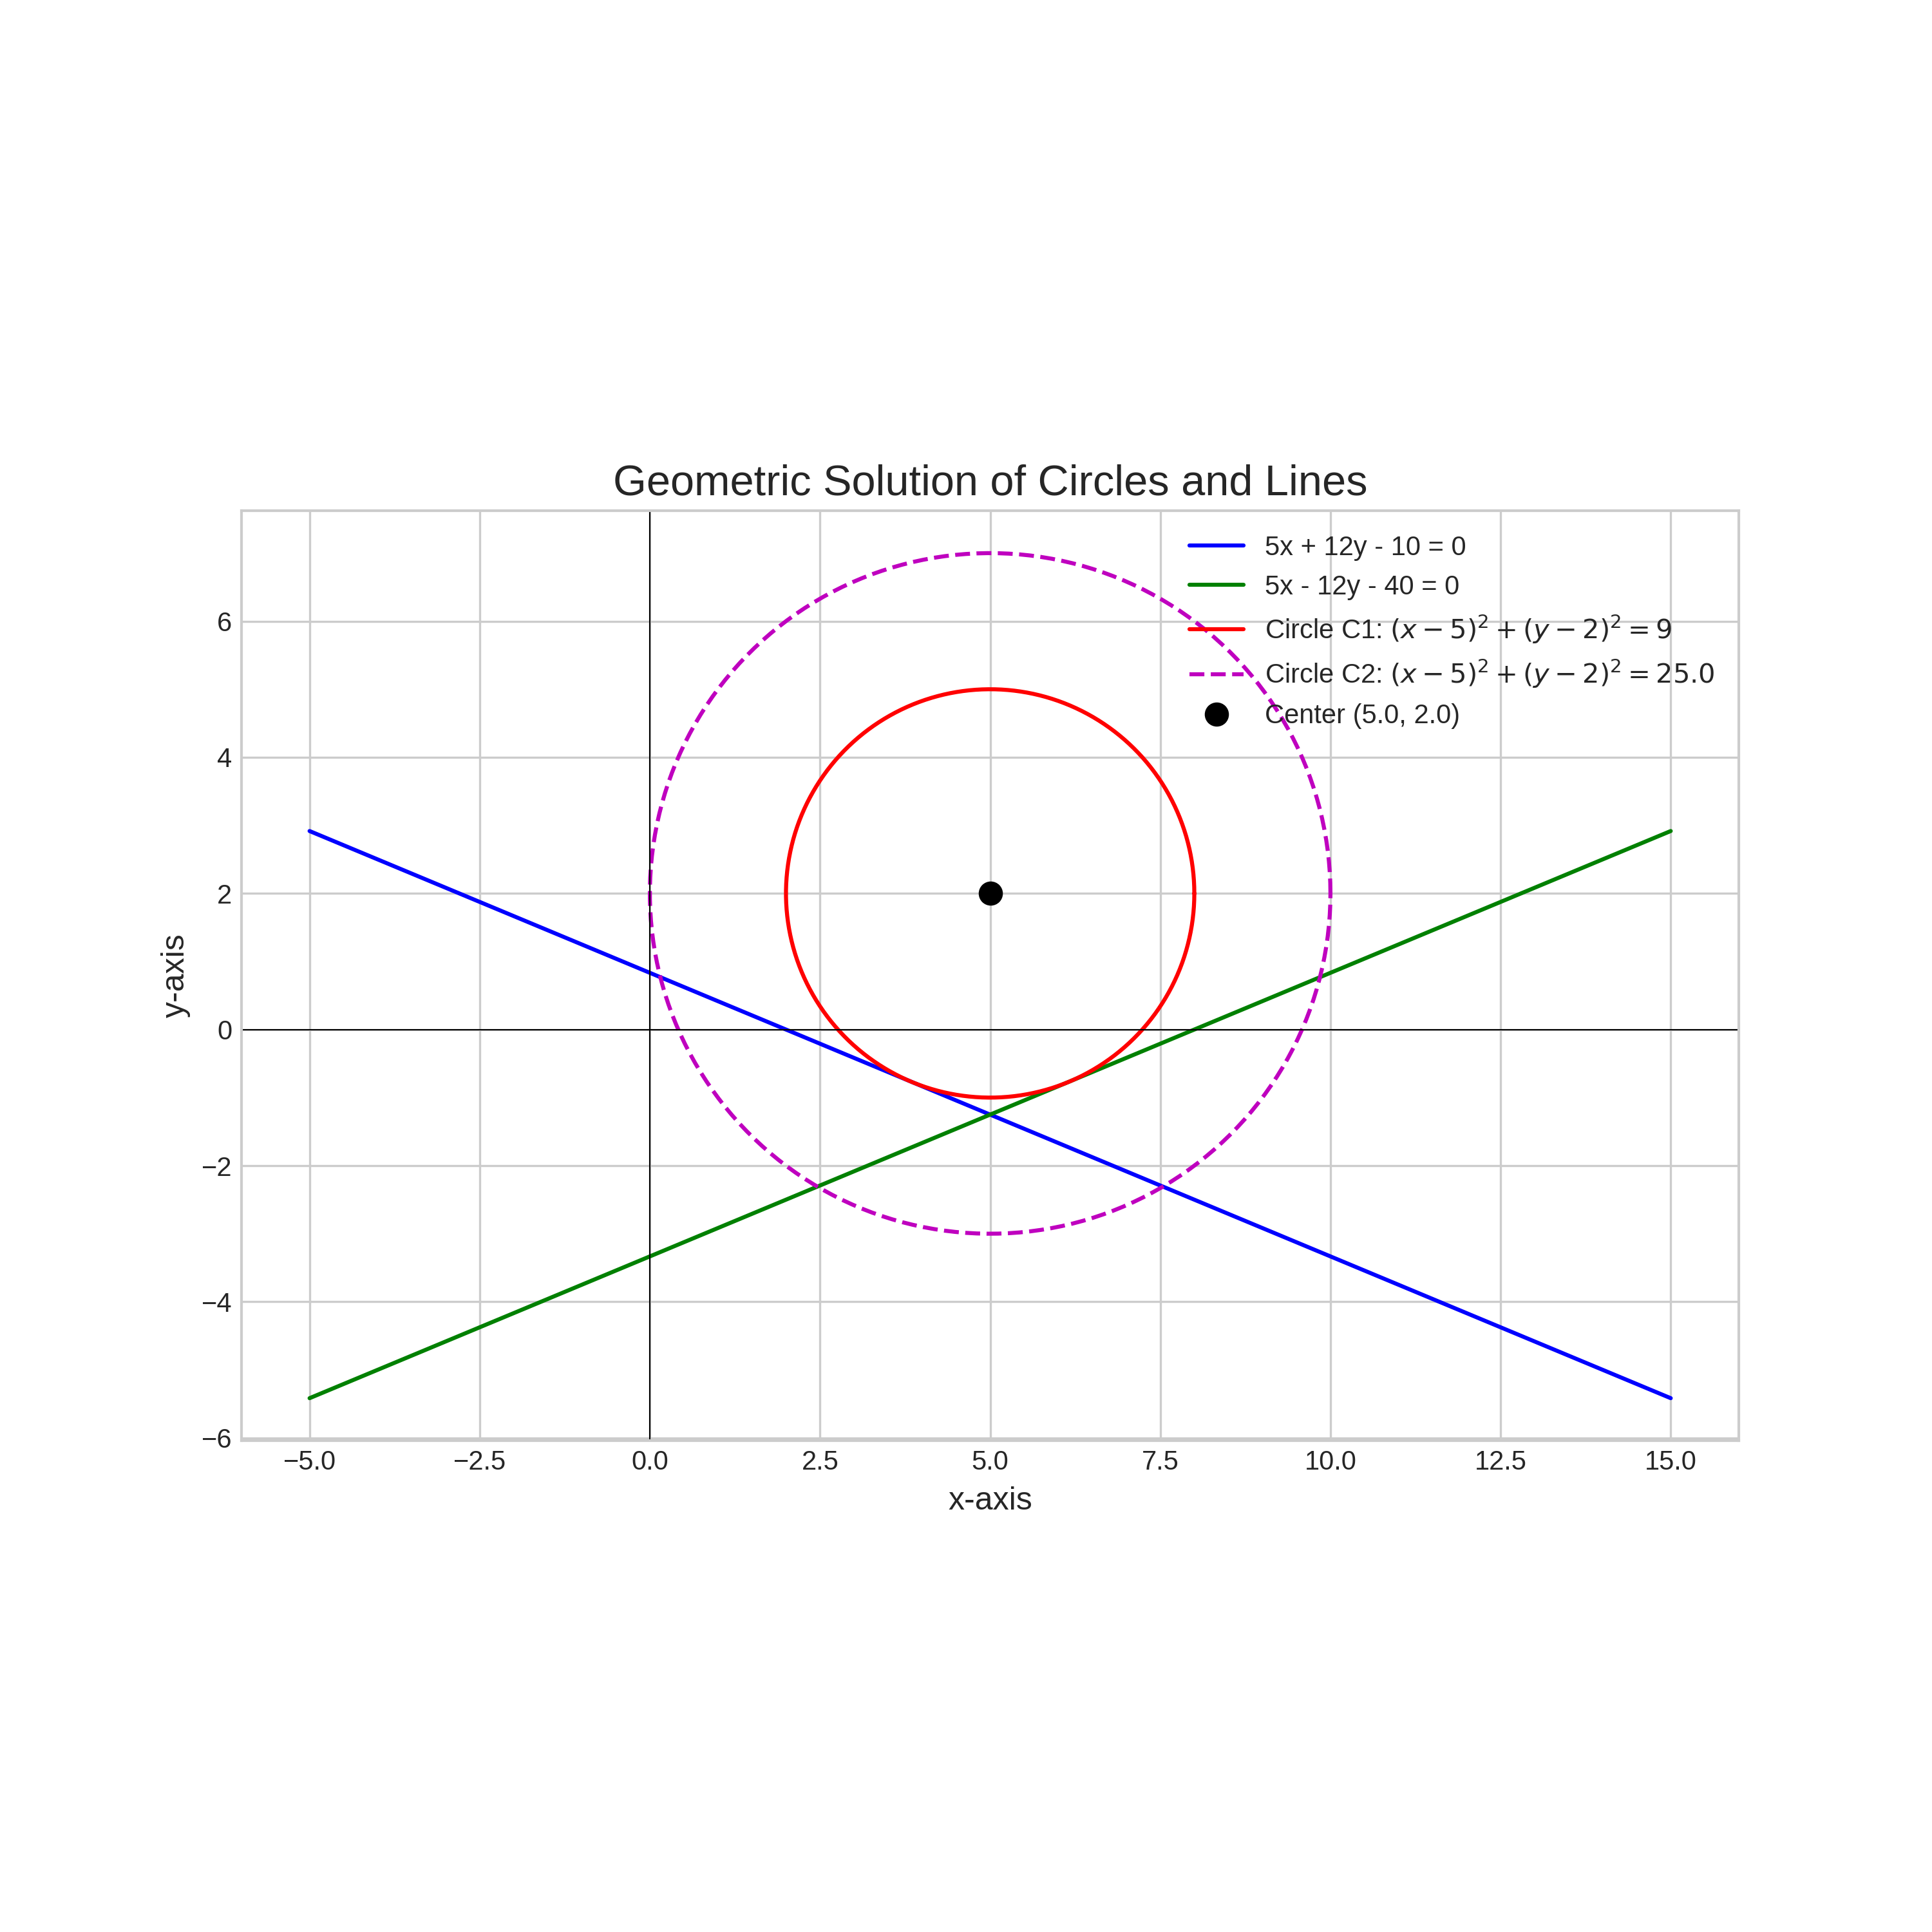
\includegraphics[width=\columnwidth]{figs/figure.png}
    \caption{}
    \label{fig:placeholder}
\end{figure}
\end{document}
